\documentclass[12pt]{article}
\usepackage[czech]{babel}
\usepackage[utf8]{inputenc}
\usepackage[IL2]{fontenc}
\usepackage{wrapfig}
\usepackage{graphicx}
\usepackage{cprotect}
\usepackage{float}


\begin{document}
%\setlength{\parindent}{0pt}
\begin{titlepage}

\includegraphics[scale=0.2, trim=5cm 0 0 30cm]{logo.jpg}
\begin{center}
\vspace{5cm}
{\Huge
\textbf{KIV/ZOS}\\
\vspace{1cm}
}
{\Large
\textbf{SEMESTRÁLNÍ PRÁCE 2017 PSEUDOFAT}
}
\end{center}
\vspace{\fill}

\begin{minipage}[t]{5cm}
\flushleft
Martin Hamet\\
A14B0254P
\end{minipage}
\hfill
\begin{minipage}[t]{7cm}
\flushright
9.února 2017
\end{minipage}
\end{titlepage}

\tableofcontents
\newpage
\section{Zadání}
\label{zadani}
Vytvoření pseudoFAT souborového systému, splňujícího následující úlohy.

\begin{itemize}
\item Nahraje soubor z adresáře do cesty virtuální FAT.

\item Smaže soubor z virtuální FAT.

\item Vypíše čísla clusterů, oddělené čárkou, obsahující data souboru.

\item Vytvoří nový adresář v zadané cestě.

\item Smaže prázdný adresář v zadané cestě.

\item Vypíše obsah souboru na obrazovku.

\item Vypíše strukturu adresářové struktury včetně souborů.

\item Zkontroluje, zda je souborový systém nepoškozen. V případě poškození zobrazí nalezené chyby a opraví je.

\end{itemize}

Omezení:
\begin{itemize}
\item Maximální počet položek v adresáři bude omezen velikostí 1 clusteru

\item Maximální délka názvu souboru bude 8+3=12 znaků (jméno.přípona) + ukončovací znak, tedy 13 bytů.

\item Každý název bude zabírat právě 12 bytů (do délky 13 bytů doplníte ukončovacím znakem - při kratších názvech).

\item Každý adresář bude zabírat přesně 1 cluster (i když nebude plně obsazen).

\item Protože se bude pracovat s velkým objemem dat, je potřeba danou úlohu paralelizovat.
\end{itemize}

\pagebreak

\section{Analýza problému a návrh řešení}
Úkolem je vytvoření pseudoFAT souborového systému. Aplikace není zamýšlena pro praktické využívání, proto není nutné zabývat se datovou kapacitou souborového systému, což usnadní ladění. Souborový systém by měl obsahovat informace o typu velikostech atp. dále pomocné struktury které budou podporovat logiku funkce a vlastní uložená data.

\subsection{Souborový systém FAT}
Budeme se držet základního principu funkce souborových systémů FAT. Tedy systém se skládá ze dvou hlavních prvků, tabulka referencí (FAT tabulka) a clusterů. Obě tyto části mohou být snadno reprezentované polem o stejné velikosti.

\subsubsection{Cluster}
Cluster je ucelený paměťový blok, pro jednoduchost pevné velikosti. Každému clusteru odpovídá jedna adresa, tedy není možné mít více clusterů než je schopné adresovat. Pro uložení dat do souborového systému se vyhradí nejmenší větší počet celých clusterů, který obsáhne daná data. Z čehož plyne problém nevhodného zvolení velikosti clusterů. Pokud bude velikost clusteru příliš malá bude potřeba vetší adresovací schopnost pro využití stejného místa. Naopak při velké velikosti clusteru se plýtvá místem. V případě souboru menšího než je velikost clusteru soubor bude fyzicky zabírat celý cluster jakožto nejmenší adresovatelnou jednotku dat.

\subsubsection{FAT tabulka}

\begin{wrapfigure}[9]{r}{9.5cm}
\centering
\vspace{-0.5cm}

Příklad uloženého souboru s obsahem \texttt{Obsah textového souboru.}
\linebreak

\begin{tabular}{|c|c|c|c|}
$\texttt{Index}$ & $\texttt{FAT tabulka}$ & $\texttt{Obsah clusteru}$\\\hline
$5$ & $6$ 				& $Obsah$\\\hline
$6$ & $9$ 				& $textového$\\\hline
$7$ & $FAT\_UNUSED$ 	& $f4fsd65faf8$\\\hline
$8$ & $FAT\_DIRECTORY$ 	& $fad5sf16af1$\\\hline
$9$ & $FAT\_END\_FILE$ 	& $souboru.$\\\hline
\end{tabular}
\caption{Příklad uložení souboru.}
\label{obr1}
\end{wrapfigure}

Jedná se o tabulku referencí na clustery. Jeden záznam v tabulce odpovídá jednomu clusteru. Funkce tabulky spočívá v poskytování informací o stavu clusteru (volný, konec souboru, adresář, poškozený). 
\\V praxi by jsme byli omezeni počtem indexů (adres). V případě číselného typu \texttt{uint8} (8 bytový integer) se jedná o maximální hodnotu 255. Z toho plyne pokud by jsme tvořili souborový systém s takovou adresovatelností mohli by jsme použít pouze 255 clusterů. Pro zaznamenání stavu clusteru budeme potřebovat 4 zmíněné hodnoty. Tedy počet adresovatelných clusterů se sníží o 4 (251 hodnot). Návaznost clusterů (např. několik clusterů obsahujících data souboru) se v tabulce projeví jako odkaz na další index clusteru v pořadí viz Obr. \ref{obr1}.

\subsection{Struktura souborového systému}
\begin{wrapfigure}[8]{r}{8.5cm}
\centering
\vspace{-0.5cm}
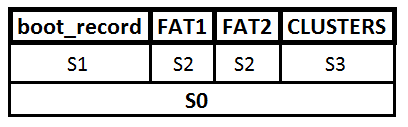
\includegraphics[width=8cm]{Structure.png}
\caption{Struktura souborového systému.}
\label{obr2}
\end{wrapfigure}
Souborovým systémem bude v našem případě myšlen výše zmíněný soubor \texttt{.dat}. V praxi takový soubor nemůže být libovolně velký a má pevně danou velikost. Tato skutečnost omezuje počet (i velikost) clusterů a tabulky. Samotné clustery jsou víceméně nepoužitelné bez příslušné tabulky, proto se tabulka v souborovém systému vyskytuje alespoň ve dvou kopiích, kdyby došlo k poškození. To znamená že je se kapacita souborového systému dále sníží viz Obr. \ref{obr2}.  Na obrázku \texttt{S0} znázorňuje celkovou velikost souborového systému. Oblast použitelná pro data je \texttt{CLUSTERS}. Z celkové velikosti musíme odečíst velikost záznamu o souborovém systému \texttt{S1}, dvakrát velikost tabulky FAT \texttt{S2}, která je daná velikostí integeru bez 4 (konstanty pro stavy clusterů viz výše) a tím získáme velikost \texttt{S3}. Z velikosti clusterů (\texttt{S3}) snadno zjistíme velikost jednoho clusteru, vydělením počtem záznamů FAT tabulky.

Pro případ naší simulace nebudeme uvažovat omezení velikosti  souborového systému \texttt{S0} a zvolíme velikost clusteru 256 bytů a počet použitelných clusterů bude 251. Neuvažujeme tedy velikosti \texttt{S1, S2}.

\pagebreak

\subsubsection{Soubor}
Soubor je tvořen řetězem referencí ve FAT tabulce viz Obr. \ref{obr1}, vlastními daty v odpovídajících clusterech a svým záznamem v příslušném adresáři (viz \ref{adresar}). Záznam v adresáři určí počáteční cluster a následující clustery lze vyčíst z FAT tabulky. Poslední soubor clusteru bude označený v tabulce jako \texttt{FAT\_FILE\_END}.

\subsubsection{Adresář} \label{adresar}
Adresář ve své nejjednodušší podobě funguje jako uzel shromažďující informace o složkách a souborech které mu jsou přiřazeny. Neobsahuje přímo jejich data ale pouze záznamy o nich. Jeho umístění v souborovém systému vyřešíme tak že vyhradíme jeden celý cluster, který ve FAT tabulce bude označen jako adresář (\texttt{FAT\_DIRECTORY}). Tento cluster bude sloužit pouze pro struktury adresáře. Adresářový cluster budeme plnit jednotlivými záznamy o souborech a dalších adresářích které obsahuje. Konkrétně viz Obr. \ref{obr3}.

\begin{figure}[H]
\centering
\begin{tabular}{|c|c|c|c|c|}
$\texttt{Záznam}$ & $\texttt{Jméno}$ & $\texttt{Soubor}$ & $\texttt{Velikost}$ & $\texttt{Počátek}$\\\hline
$1$ & $soubor1$ & $True$	& $100B$ & $2$\\\hline
$2$ & $soubor2$ & $True$	& $200B$ & $5$\\\hline
$3$ & $složka1$ & $False$	& $0$	 & $8$\\\hline
$4$ & $složka2$ & $False$	& $0$	 & $9$\\\hline
\end{tabular}
\caption{Příklad adresářového clusteru.}
\label{obr3}
\end{figure}

V každém záznamu je uvedeno zda se jedná o záznam souboru (\texttt{True}) nebo dalšího vnořeného adresáře (\texttt{False}). V případě souboru i jak je soubor velký. Toho využijeme při čtení souboru, protože máme pouze informaci o jemu přiřazených clusterech. Díky velikosti zjistíme kolik z místa soubor zabírá ve svém posledním clusteru. V obou případech záznam obsahuje počátek, který určuje index clusteru, kde začínají data daného záznamu. Díky této struktuře bude možné rozvětvovat strom adresářů pouze s omezením počtu volných clusterů.

Záznam v adresářovém clusteru bude zabírat pevně danou velikost. Z toho plyne omezení počtu záznamů na adresář. Jinak by adresář přesahoval svůj přidělený cluster (počátek) a bylo by nutné situaci řešit jinak.

Aby bylo možné vkládat soubory a složky bude v základu vytvořen adresář \texttt{root} na prvním clusteru ze kterého se bude vždy vycházet.

\subsection{Informace o souborovém systému}
Podle vzoru bude vhodné zavést strukturu \texttt{boot record} která by měla obsahovat veškeré základní informace o souborovém systému (popis, typ, počet fat tabulek, velikost clusteru, počet použitelných clusterů). Tento záznam by se měl vyskytnout na začátku souboru \texttt{.dat} (souborového systému).

\subsection{Kontrola souborového systému}
Snaha je o udržení souborového systému v co nejlepším stavu a především zabránit ztrátě dat. Je nutné tedy kontrolovat konzistenci souborů a záznamů o nich podobně jako adresářů. Systémovým chybám lze předejít např. logováním (tvoření žurnálu o změnách). V naší simulaci se ale zaměřím spíše na opravu již vzniklých chyb.

\subsubsection{Hledání chyb}
Pro hledání chyb lze použít různé metody v této práci sem zvolil pouze několik základních principů.

\paragraph{hit test}
Jako hlavní metodu odhalování chyb jsem zvolil hit test. Nejprve bude nutné vytvořit pole čítačů (pro každý cluster jeden čítač). Metoda spočívá v rekurzivním průchodu adresářové struktury z kořenového adresáře a zvýšení příslušného čítače při objevení záznamu (adresář, soubor). U souboru je nutné zvýšit čítač u každého clusteru který je mu přidělený. Výsledkem je pole znázorňující kolikrát byl každý cluster nalezen. Porovnáním tohoto výsledku a záznamů ve FAT tabulce můžeme vyvozovat různé chyby viz \ref{oprava}.

\paragraph{vlastnosti souboru}
Je možné odhalit neukončený soubor podle jeho záznamu o velikosti nebo tvaru jména (duplicita, délka). Pokud velikost všech přidělených clusterů přesahuje velikost v záznamu souboru. Případně pokud by soubor jako svůj další cluster odkazoval na adresář nebo na nevyužitý cluster.

\pagebreak

\paragraph{sekundární FAT tabulka}
Při rozdílných záznamech v primární a sekundární FAT tabulce. Bohužel se již dále bude hůře určovat, která tabulka je chybná proto se budu spíše spoléhal na tabulku primární a v případě podezření na chybu kontrolovat s tabulkou sekundární. Je značně nižší šance že se náhodná chyba projeví v obou tabulkách. Při neshodě tabulek by mohlo být užitečné soubor ukončit a pokusit se z clusterů bez reference vytvořit samostatný soubor.

\subsubsection{Oprava chyb} \label{oprava}
Při opravování chyb nelze vždy určit správný postup a rozhodování není triviální proto se budeme držet jednodušších mechanismů.

Za nejužitečnější nástroj bych považoval výše zmíněný hit test.
\paragraph{Případy hit testu:}
\begin{itemize}

\item \textbf{odkaz na nepoužitý cluster} Předpokládáme správnost odkazu a pokusíme se podle typu odkazu obnovit adresář nebo soubor. V případě obnovení adresáře hrozí že se obnoví množství neplatných souborů pokud bude obsahovat platné adresy. Tento problém se nedá předem odhalit a proto bych se o obnovu radši pokusil. Aby nedocházelo k takovému stavu často proběhne nejprve kontrola obou tabulek, a obnovení proběhne pouze v případě, že obě tabulky obsahují stejný záznam. Tedy v obou je daný cluster označen jako např. jako adresář.

\item \textbf{násobný odkaz na adresář} V běžném souborovém systému by to nebyla chyba (linkování atp.), v našem případě ale duplicitní odkaz odstraníme. Zabráníme tím násobnému opravování souborů ve vnořených adresářích. Podobně jako u datového clusteru bude rozhodnutí o znovuzavedení adresáře záviset na shodě FAT tabulek.

\item \textbf{adresář bez reference} Ztráta reference na adresář by se měla vždy řešit pokusem o obnovu. Vytvoření nového adresářového záznamu s odkazem na nalezený cluster v kořenovém adresáři. Tato operace vyžaduje nový hit test z toho důvodu, že adresář mohl obsahovat další záznamy a bude lepší je hned zahrnout do testování než se je pokoušet obnovit "na slepo".

\pagebreak

\item \textbf{násobná reference na cluster} Jedná se pravděpodobně o křížení souborů. Aby nedošlo k poškození ani jednoho z nich (pokud je některý v pořádku) bylo by vhodné najít soubory, kterým zmíněné clustery patří a vytvořit kopii. Jeden soubor zkopírovat na nové místo, aby se při jejich další změně nepřepisovali data obou. Vzhledem k tomu že v naší simulaci není možné uložené soubory přepisovat tak tuto opravu pominu z důvodu komplikovaného rozhodování v kombinaci s ostatními chybami. Křížení budeme řešit pomocí záznamu hit testu a pokud by nastala "potkání" clusteru který už byl zaznamenán v hit testu ukončíme právě zkoumaný soubor.

\item \textbf{datový cluster bez reference} Mohlo by se jednat o soubor na který se ztratila reference. Pokračováním podle návaznosti dle FAT tabulky by mohlo zapříčinit "roztrhání" souboru na několik nalezených. Proto bude lepší řešit tyto případy na konci kontroly, kdy už víme o všech clusterech tohoto typu. Z množiny těchto clusterů se pokusíme podle FAT tabulky sestavit co nejdelší řetězce vedoucí ke konci souboru. Těmto řetězcům dále vytvořit záznamy v kořenovém adresáři.
\end{itemize}

\pagebreak

\paragraph{Ostatní případy:}
\begin{itemize}
\item \textbf{záznam o souboru odkazuje na nevalidní cluster} Naše struktura neobsahuje zálohy adresářů. Není tedy kde začít a záznam o souboru bude smazán. 

\item \textbf{soubor v průběhu obsahuje odkaz na nevalidní cluster} V případě že nevalidní cluster je adresář bude soubor ukončen záznamem \texttt{FAT\_FILE\_END} na svém předchozím clusteru aby nedošlo k poškození dalších souborů. V ostatních případech je možné zkontrolovat stav se sekundární FAT tabulkou a nahradit záznam v primární, jinak bude soubor ukončen.

\item \textbf{počet clusterů souboru neodpovídá jeho velikosti} Soubor bude ukončen primárně podle své velikosti aby se zabránilo poškozování dalších souborů.

\item \textbf{dva záznamy ve stejném adresáři mají stejný název} Prvnímu takovému záznamu s duplicitou bude vygenerováno nové jméno.

\item \textbf{název záznamu neodpovídá standardu} Standardní velikosti jména je 12 znaků včetně tečky oddělující třípísmennou koncovku. Nestandardnímu souboru bude vygenerováno nové jméno s ohledem na duplicitu.
\end{itemize}

\pagebreak

\section{Implementace}
Program je připraven na případnou změnu na jinak velký souborový systém nicméně některé součásti jsou závislé na zvoleném typu souborového systému podle vzoru FAT8.

\subsubsection{Hlavní části programu} 

\paragraph{\texttt{main}}
Zajišťuje zpracování předaných parametrů načtení \texttt{(load\_fat)} a uložení \texttt{(save\_fat)} souborového systému a volání příslušných funkcí podle přepínačů.

\paragraph{\texttt{import\_file}}
Zajistí načtení souboru \texttt{(load\_file)} z disku vytvoření příslušného záznamu \texttt{(create\_file\_rec)} podle zadané adresy a uložení do souborového systému.

\paragraph{\texttt{create\_directory}}
Zajistí vytvoření adresáře a jeho záznamu \texttt{(create\_directory\_rec)} podle zadaných parametrů.

\paragraph{\texttt{get\_directory\_cluster}}
Slouží ke zpracování zadané adresy do souborového systému a získání příslušného indexu adresářového clusteru.

\paragraph{\texttt{get\_record}}
Z adresy do souborového systému získá ukazatel přímo na hledaný záznam \texttt{(get\_directory\_cluster), (get\_node\_offset)}.

\paragraph{\texttt{check\_structure}}
Zajišťuje hlavní kontrolu souborového systému \texttt{(hit\_test\_arr)}. Poskytuje obecné informace o kontrole. V případě potřeby spouští obnovu nalezených souborů a adresářů\texttt{(recover\_directory), (file\_recovery)}.

\paragraph{\texttt{hit\_test\_arr}}
Rekurzivně prochází adresářovou strukturu a zaznamenává nalezené soubory a složky \texttt{(mark\_directory), (mark\_file)} do záznamu hit testu. A provádí vedlejší kontroly (jméno, velikost, validní odkazy atp.) a příslušné opravy.

\paragraph{\texttt{file\_recovery}}
Po dokončení ostatních oprav prochází finální výsledky hit testu a tvoří list zřetězených clusterů které k sobě patří (dle FAT tabulky referencí). Po dokončení průchodů založí záznamy, pro každý řetězec ( potencionální soubor) v kořenovém adresáři.

\section{Uživatelská příručka}
Program je určen pro spouštění z příkazové řádky. Podle zadaných parametrů vykonává požadované funkce nad souborem \texttt{.dat}.

\subsubsection{Ovládání programu (přepínače)}

\paragraph{\texttt{ZOS\_FAT.exe soubor.dat -a S1 ADR}}
Nahraje soubor z adresáře do cesty virtuální FAT tabulky.
\\S1 soubor pro nahrání
\\ADR adresa do souborového systému

\paragraph{\texttt{ZOS\_FAT.exe soubor.dat -f S1}}
Smaže soubor S1 ze soubor.dat.
\\S1 plná cesta k souboru 

\paragraph{\texttt{ZOS\_FAT.exe soubor.dat -c S1}}
Vypíše čísla clusterů, oddělené dvojtečkou, obsahující data souboru S1.
\\S1 plná cesta k souboru 

\paragraph{\texttt{ZOS\_FAT.exe soubor.dat -m ADR ADR2}}
Vytvoří nový adresář ADR v cestě ADR2.
\\ADR název nového adresáře
\\ADR2 cesta pro nový adresář

\paragraph{\texttt{ZOS\_FAT.exe soubor.dat -r ADR}}
Smaže prázdný adresář ADR.
\\ADR cesta k adresáři

\paragraph{\texttt{ZOS\_FAT.exe soubor.dat -l S1}}
Vypíše obsah souboru S1 na obrazovku.
\\S1 plná cesta k souboru

\paragraph{\texttt{ZOS\_FAT.exe soubor.dat -p}}
Vypíše adresářovou strukturu s odpovídajícím odsazením.

\paragraph{\texttt{ZOS\_FAT.exe soubor.dat -s}}
Provede kontrolu, případné opravy a výpis výsledku.

\paragraph{\texttt{ZOS\_FAT.exe soubor.dat -e}}
Vytvoří nový soubor empty.dat s prázdným souborovým systémem.

\section{Závěr}
Parametry souborového systému byli zvolené tak, aby bylo snazší ladění což se projevilo jako výhoda. Jednotlivé úkoly nebyly náročné na implementaci po připravení základní funkčností systému. Naopak značné problémy způsobovala kontrola a oprava souborového systému. Opravy i kontrola by šla výrazně vylepšit, ale náročnost hledání a opravování chyb rychle roste. S novými způsoby oprav přibývají možnosti poškození ostatních struktur a je třeba komplexnější rozhodování. Přesto se podařilo připravit program na detekci a opravu jednoduchých chyb. Program je schopen obnovit ztracené adresáře, soubory a srovnat nebo částečně opravit neukončené soubory. Přerušené soubory je program schopen detekovat a obnovit alespoň jako dva nezávislé.

Paralelizace načítání a ukládání souboru se po hlubším zkoumání projevila jako téměř zbytečná, při uvážení plnění bufferu jedním vláknem a zpracování dat z bufferu ostatními, protože místo bufferu může vlákno ukládat data rovnou na požadované místo. Paralelní zpracování by tedy přicházelo v úvahu pro kontrolu souborového systému což se projevilo jako poměrně náročný úkol a z časových důvodů jsem tuto variantu zavrhl.

\end{document}